\documentclass{report}
\usepackage[utf8]{inputenc}
\usepackage{blindtext}
\usepackage{graphicx}
\usepackage{indentfirst}
\usepackage{pdflscape}
\usepackage{pdfpages}
\usepackage{verbatim}
\usepackage{listings}
\usepackage{amsmath}
\usepackage{amsfonts}
\usepackage{amssymb}
\usepackage{geometry}
\usepackage{tikz}
\usetikzlibrary{calc}


%
\makeatletter
\setlength{\@fptop}{0pt}
\makeatother

\usepackage{geometry}
 \geometry{
 a4paper,
 total={170mm,257mm},
 left=20mm,
 top=20mm,
 }
 
 
\begin{document}
%----------------------------------------------------------------------------------------
%	HEADING SECTIONS
%----------------------------------------------------------------------------------------
\newcommand{\HRule}{\rule{\linewidth}{0.5mm}}
\begin{titlepage}
   \title{
       \large{Master 1 Computer Science}
       \HRule\\
       \LARGE\textbf{Memoire}
       \HRule\\
       \textsc{Génération de modèles de réseaux de neurones} % Title of the report
   }
   
   
   \author{\\Théo Maria\\Brian Dietrich\\Brian Lebreton\\Emmanoe Delar\\Najeebullah Ahmadzai}
   
   \nointerlineskip
   \vfill
   \let\snewpage \newpage
   \let\newpage \relax
   \maketitle
   \let \newpage \snewpage
   
   \center
 
   \textsc{Clients : Linh Van Le and Marie Beurton-Aimar}
   
   \textsc{Teacher : Adrien Boussicault}
   
   
\includegraphics[scale=0.2]{figures/logo.jpg}\\
   \break
   \vfill

\end{titlepage}


%---------------------------
%----------Table of contents
%---------------------------
 
\tableofcontents

\newpage

%---------------------------
%--------- Chapter 1 -------
%---------------------------

\chapter{Presentation of the project}
\section{Introduction}

 The goal of our programming project is about developing a Python-based GUI (Graphical User Interface) that interfaces PyTorch; an open-source deep learning frameworks.
 \newline Like Expresso for Caffe, NVidia DIGITS for Theano, Caffe, Torch and Tensorflow. A lot of graphical user interface which provide numerous tools for deep learning frameworks are available. Unfortunately they are not compatible with the PyTorch Library at the time when we begin this project. So, the alternative we propose is an application that will be an interface for PyTorch and gives the abilities to use all the deep learning features provided by the Pytorch framework.
 \newline Our application goal is to provides interesting features with manipulation of neural network. It will also integrate Jupyter-Notebook thus user could expereience live coding, graph computation and specifically neural network vizualisations. 


\begin{figure}[!ht]
    \center
    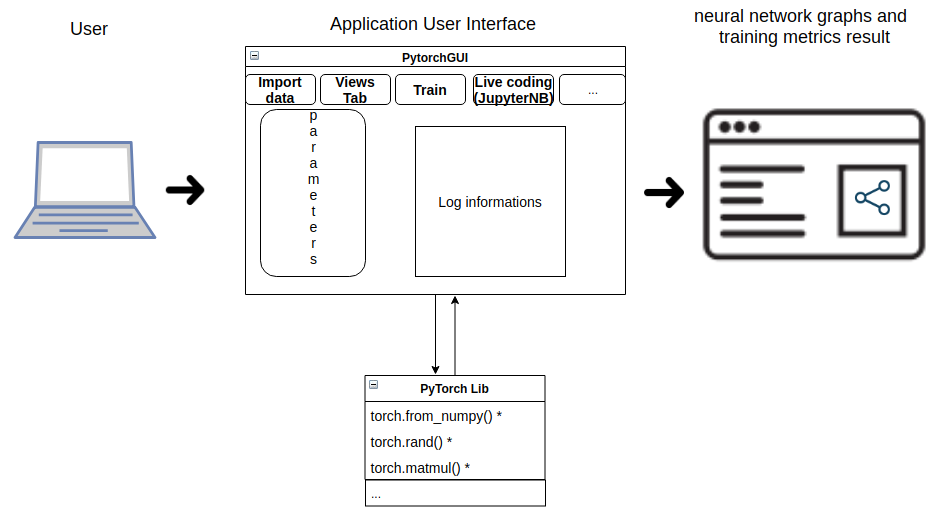
\includegraphics[scale=0.4]{figures/schema_intro1.png}
    \caption{Schematic view of the project}
\end{figure}
\footnote{Features shown in this schema will be discuss further below}

\section{Definitions}
Before we dive in the project code implementation and it's architecture let us start with some fundamentals in Artificial Intelligence and examples.

\subsection{Artificial Intelligence, Machine learning and Deep Learning}
In the early days, of AI, algorithms were used to solve problems that where difficult for humans to solve. Machine were hard coded, such as a computer program playing chess.
\newline Machine learning is one of the fields of study of Artificial Intelligence. It relies on statistical concepts as well as models to give machines the ability to learn. It basically consists of showing a lots of examples, using a set of data, the training set, to make our algorithm try to recognize patterns in it, so it can learn to recognize new data instantly thus come up with rules to predict outcomes for unseen data:

\begin{figure}[!ht]
    \center
    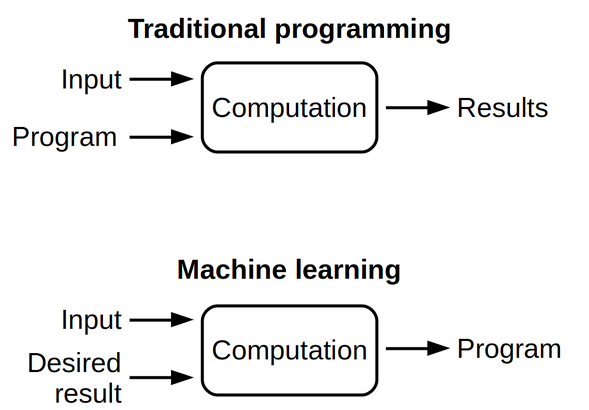
\includegraphics[scale=0.3]{figures/marchine_learning_para.png}
    \caption{Traditional Programming vs Machine Learning}
\end{figure}


The training phase of a machine learning algorithm takes the training set, and tries for a pre-determined number of iterations, to classify the data. In each iteration, the algorithm will take into account the errors of classification in the last iteration to correct itself, step by step, until its accuracy is high enough.

There are different types of approach for machine learning algorithms :
\begin{itemize}
\item Supervised learning : In this case, the data is annotated, which means the algorithm knows the inputs and the outputs of the set. It allows to directly check if the result is correct in each iteration.
\item Semi-supervised learning : In this case it's the same as supervised learning, with the exception that only a part of the data is annotated
\item Unsupervised learning : This type of approach is clearly distinct from the two others, since the data is not annotated. In this case, the algorithm will try to find patterns by itself, without the use of external corrections. It's only after training that the user can see the results.
\end{itemize}

Once the training of the algorithm is finished, we can evaluate it by using another data-set, which contains different data than the training set, to evaluate the accuracy of our algorithm. \usetikzlibrary{}Here is a visualization among AI, ML and DL.

\begin{figure}[!ht]
    \center
    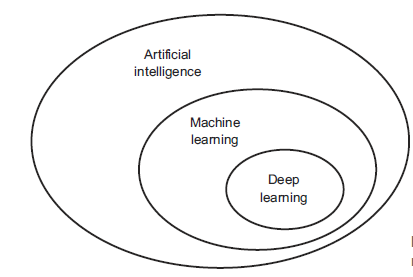
\includegraphics[scale=0.5]{figures/aivsmlvsdl.png}
    \caption{About AI}
\end{figure}

Deep Learning algorithms are a part of the machine learning family algorithms. To be able to recognize patterns in data, they use a cascade of multiple layers of nonlinear processing units. Each layer uses the output from the previous one. They work with the concept of deep neural networks.

\newpage
\subsection{PyTorch}
In Pytorch, data are represented as tensor or variable.
\subsubsection{Tensor}
Tensor are Python's numpy array but they can be used with GPU. In our project we will not use the GPU but the CPU, we still working on this feature it will be avaible in newer version of the app. But tensor still useable with CPUs. 
\newline Like arrays, tensors contains elements and can be multidimensional. Frequenntly used tensor are :
\begin{itemize}
    \item Scalar (0-D tensors)
    \item Vector (1-D tensors)
    \item Matrix (2-D tensors)
    \item 3-D tensors
    \item Slicing - tensors
    \item 4-D tensors
    \item 5-D tensors
\end{itemize}

For example, image can be represented as 3D-Tensor (height,weight, channel (RGB)) so a 4D-Tensor can be a Tensor with a batch of images. The number of images are represented in the 4th dimension. Slicing tensor are one-dimensional tensor that we slice the elements. For example 1-D\_tensor\textit{[:slice\_index]}   

\subsubsection{Variables}
Pytorch variables can be seen as containers with:
\begin{itemize}
    \item Data : tensor object
    \item Gradients
    \item Creator: reference to the function that created it
\end{itemize}

\subsection{Computation graphs}
To represent deep learning algorithms we can use graphs. The following computational graph computes the sum z of two inputs x and y:

\begin{figure}[!ht]
    \center
    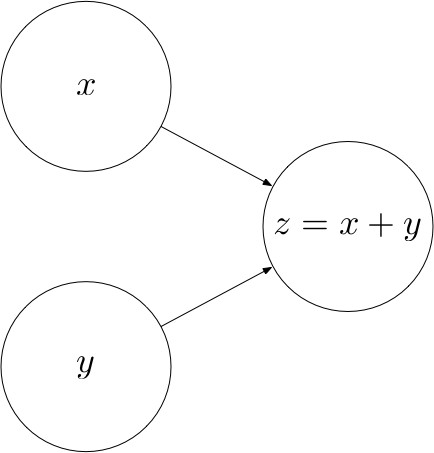
\includegraphics[scale=0.4]{figures/computational_graph.png}
    \caption{Representation of a computational graph }
\end{figure}

Here, x and y are input nodes to z and z is a consumer of x and y. 
\subsection{Neural network model}
To build a model wich learns how to map the outputs from the inputs we must learn the network (functoin) by showing the inputs and the associated output. For a linear relationship model represented as y = wx + b. Here is its associated computation graph:

\begin{figure}[!ht]
    \center
    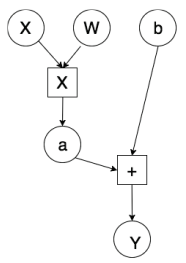
\includegraphics[scale=0.8]{figures/linear.png}
    \caption{Linear relationship graph }
\end{figure}

\subsubsection{implementation}
\begin{lstlisting}
def linear_model(x):
    y = torch.matmul(x,w)
    return y
\end{lstlisting}

\subsection{Layer}
\subsubsection{torch.nn}
Pytorch provides a higher level abstraction in torch.nn called layers wich create latyer much simpler.
\begin{lstlisting}
class torch.nn.Linear(in_features, out_features, bias=True)
\end{lstlisting}
Applies a linear transformation to the incoming data: y=Ax+b
\newline Parameters:	
\begin{itemize}
    \item in\_features – size of each input sample
    \item out\_features – size of each output sample
    \item bias – If set to False, the layer will not learn an additive bias. Default: True
\end{itemize}

\noindent The previous model can be represented as a torch.nn layer as follow:
    \begin{lstlisting}
    f = nn.Linear(17,1) 
    \end{lstlisting}

\subsection{Loss function}


%---------------------------
%--------- Chapter 2 -------
%---------------------------
\chapter{Tools}
To lead this project to the end, we are going to use some tools that will help us accomplish this project.

\section{PyTorch library}

PyTorch is an open-source machine learning library for Python. It is based on Torch, which is an old machine learning library (first release : October 2002), itself based on the Lua programming language. PyTorch library allow users to be able to create neural networks, edit existing models, and make calculations on those networks with high-level abstraction functions.

A neural network is a collection of neurons interconnected and permits the resolution of complex problems like graphical recognition or the natural language treatment by the blessing of the  of the weighting adjustment coefficients in a learning phase.
The idea of the program is to read a file (list in Elicitation Requirements), choose an algorithm, edit its parameters then perform a calculation thanks to PyTorch then it returns different results depending the different parameters you entered previously. Results can be found in the form of pictures edited from the original, graphs and statistics data.
\newline This application can be used by anyone wishing to use the PyTorch Deep Learning Library experiment and create models. Users can be scientist, students, everyone that is interested in Deep Learning practice

\section{HiddenLayer library}
HiddenLayer is a A lightweight library for neural network graphs and training metrics for PyTorch, Tensorflow, and Keras developed by Waleed Abdulla  and Phil Ferriere, and is licensed under the MIT License.
\newline We choose to use this library to render graphs of neural networks and export them as pdf or png files.

\section{Jupyter NoteBook}
HiddenLayer work with jupyter notebook. Jupyter Notebook is a great tool for data scientist. We will use it in background of our applciation for graph computing data representation and training metric. It provide us, a great background environment. 
\section{Integrated development environment}
We all have our familiarities with some integrated development environment (IDE).
This are those we will most likely be using : 
    - Emacs
    - Atom
    - Sublime Text
    - Visual Studio Code
    - Qt Creator

\section{Libraries}
We will use some libraries that will ease us the task. Those libraries might change over the progress of our project :
\begin{itemize}
    \item PyTorch 
    \item Qt: Since we plan on using QT Creator to create our graphical interface, we will surely make use of the QT Library, which provides a lot of graphical elements.
    \item Plotly: Using this library could be very useful. It can indeed provide a lot of graphical features, like plotting data, and generating graphs.
    \item Numpy: Numpy is an extension to the Python language, which allows to manipulate matrices and multidimensional arrays, and to use a variety of mathematical operations on it. Numpy is already integrated to PyTorch.
    \item Networkx: A python library for studying graphs and networks.
    \item h5py: Our application needs to be able to read hdf5 files. This library allows to read them.
\end{itemize}

\section{Utilities}

\begin{itemize}
    \item Version control system (VCS)
        As we work as a group and not individually on totally independent tasks, we have to use a VCS. Since we all know GitHub, we chose to use this simple VCS.
\end{itemize}


%---------------------------
%--------- Chapter 3 -------
%---------------------------
\chapter{Existing Analysis}
For ideas and inspiration, we analyzed the existing projects, resources and their interrelated materials.

\section{Caffe and Expresso}

\subsection{Caffe}
Caffe (which stands for Convolutional Architecture for Fast Feature Embedding) is an open source deep learning framework, originally developed at University of California, Berkeley. 

\subsection{Expresso}
Expresso has been developed, to graphically control Caffe library. The framework itself is written in C++, but it has a python interface.

\noindent Expresso is a Python-based graphical user interface made for designing, training, and exploring deep-learning frameworks. It is built atop of Caffe. Its main purpose is to facilitate the use of Caffe by providing a user interface which allow to use most of its features graphically.\\

\noindent Expresso has a handy importing tool which enables users to import different formats of data such as Text, LevelDB, .mat, HDF5 and Folder formats. It provides additional information regarding to the data being imported in a detailed manner.
A technical browser tool is provided, which can be used for a quick preview of the imported data.
The imported data can be exported to the other formats. 

\noindent Another interesting feature is that the back-end framework related to Data view also features a parser. This parser can be utilized to quickly extend the import interface to load data in formats not provided yet in Data view.

\noindent Expresso interface is separated into four different views : Data View, Net View, Train View and Exp View
These different views will basically be our main inspiration for how we organize our application.
\begin{itemize}
\item Data view allows to import data, by selecting the format of the file. In addition, it provides support for basic data manipulation. The back-end framework of data view also allows to program a new import functionality, which allows to import formats that are not supported yet.
\item Network view is used to design a deep network from scratch. Each layer of the network can be created and modified using an edit interface, which automatically provides contextual layer description, as the user types. They are color-coded by type, for easy visualization. The "train net" tab allows to create a net, and the "deploy net" tab allows to modify an existing one. All the created networks are Caffe-compatible, which means the user can use them outside of Expresso as well.
\item The train view is used to train the deep networks. Expresso allows training to be stopped midway, and resumed. In addition to conventional deep network training, it also allows provides support for training external classifiers. These classifiers are trained on features obtained by passing data through trained net.
\item Experiment view can be used for three important tasks :
\begin{itemize}
\item Feature extraction using featuring nets : In the deep-learning field, a "feature" is basically a pattern that can be found in a set of data. For example, it can be used to distinguish shapes in pictures. Feature extraction is a process that consists of finding the features.
\item Visualizing feature data : This basically allows to visualise the features found in an image, with the use of colors
\item Testing pre-trained models : Once a model is trained with the use of a training data-set, it can be tested with another data-set. By this process, we can determine the accuracy of a model, which will allow to compare it to other models.
\end{itemize}
\end{itemize}
The Expresso application is multi-threaded, which means it can enable concurrent execution of tasks. It provides a notification system, which can alert the user when there is an event, or when a task is completed.

All of the screen captures of the application can be found later in \textbf{Annexes}.

\begin{comment}
\begin{figure}[!ht]
\center
    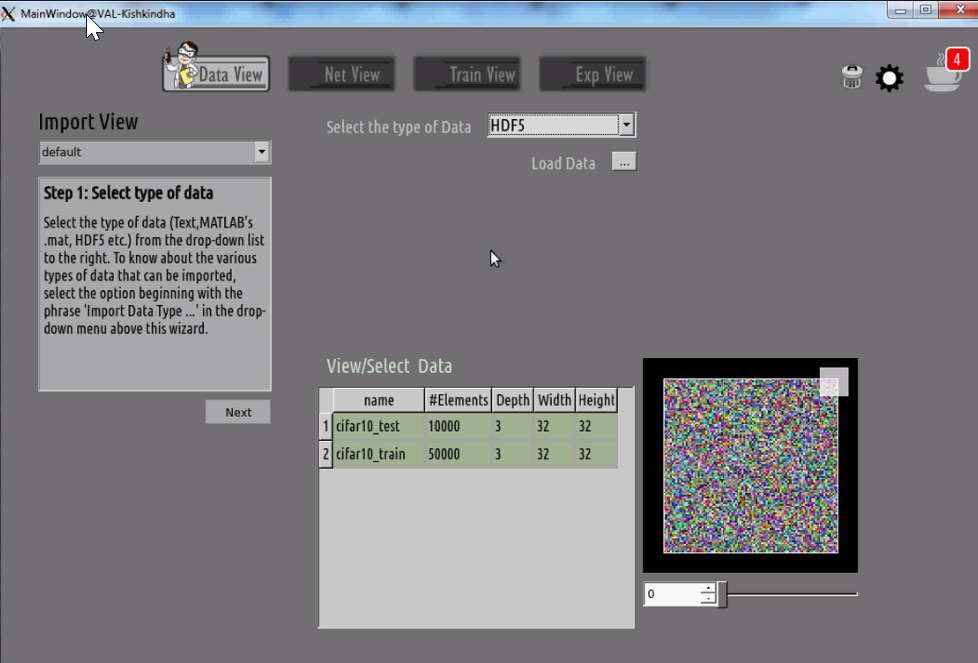
\includegraphics[scale=0.8]{images_expresso/01_data.png}
    \caption{Expresso Data View}
\end{figure}

\begin{figure}[!ht]
\center
    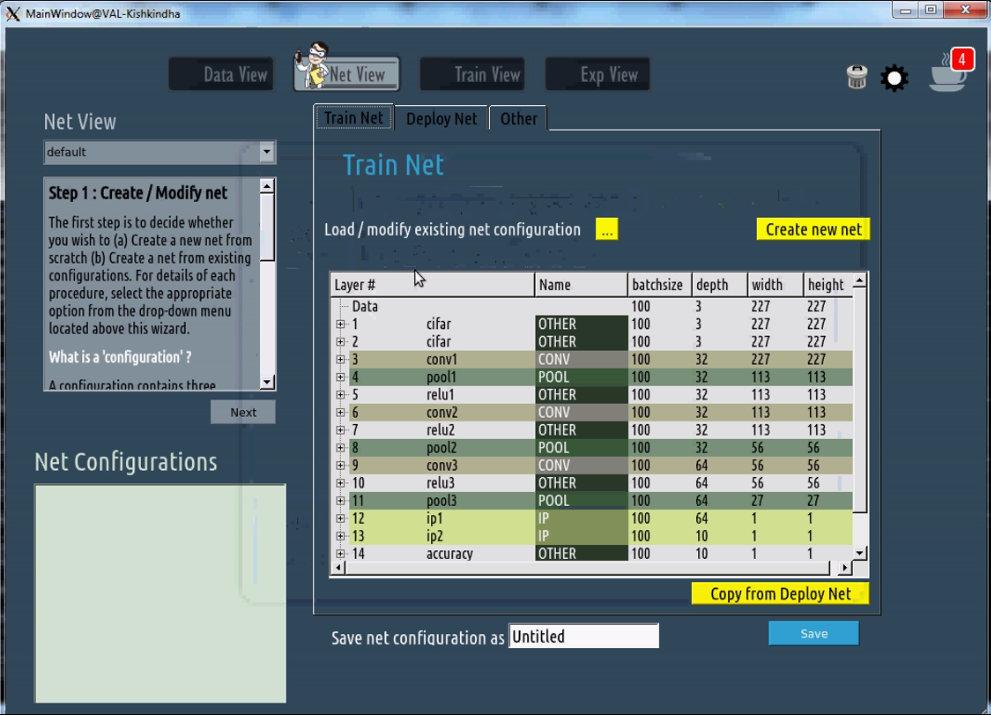
\includegraphics[scale=0.8]{images_expresso/02_net_train_net.png}
    \caption{Expresso Network View}
\end{figure}

\begin{figure}[!ht]
\center
    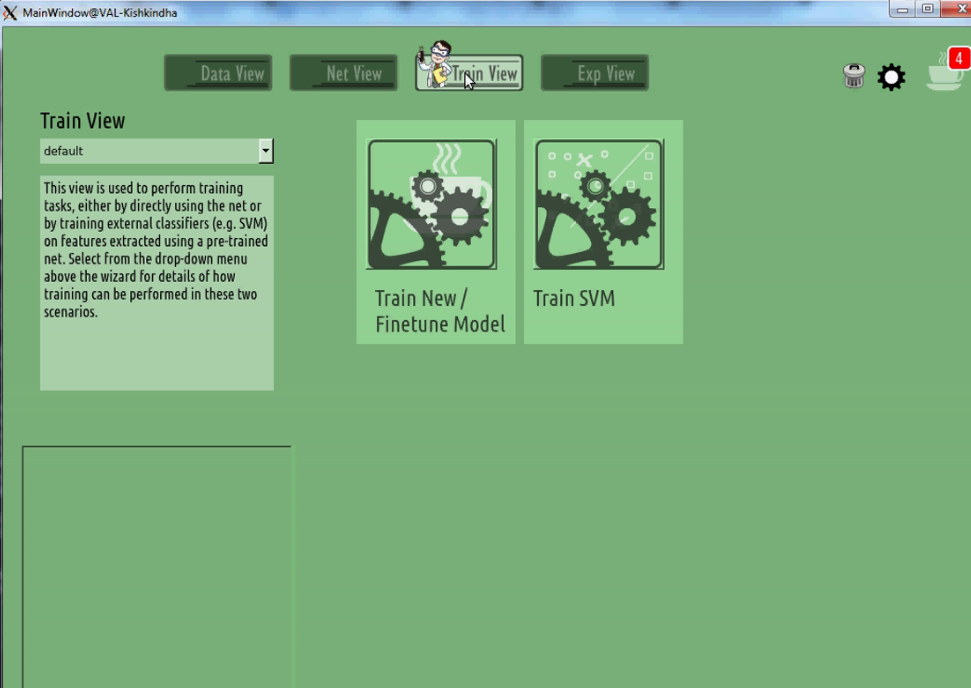
\includegraphics[scale=0.8]{images_expresso/05_train.png}
    \caption{Expresso Train View}
\end{figure}

\begin{figure}[!ht]
\center
    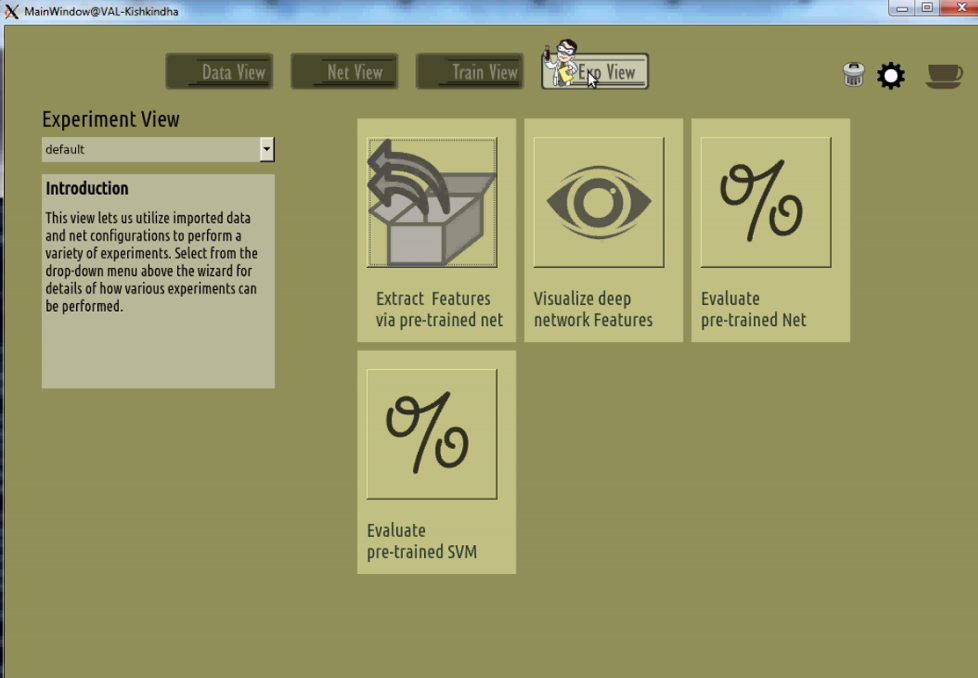
\includegraphics[scale=0.8]{images_expresso/09_exp.png}
    \caption{Expresso Experimental View}
\end{figure}
\end{comment}

\section{Keras}
Keras is an open source neural network library written in Python. It can run on top of many popular neural network software, like TensorFlow or Microsoft Cognitive Toolkit.
It was initially released in March 2015. It mainly allows to facilitate working with image and text data by adding commonly used network models.

\section{Tensorflow}
TensorFlow is an open-source software library of dataflow programming across a range of tasks. It was originally developed by the Google Brain team, and was first released in November 2015.
It is used for all kind of math computation, but it's features allow to use it for machine learning.



%---------------------------
%--------- Chapter 4 -------
%---------------------------
\chapter{Requirements Elicitation}
\section{PyTorchGUI}
\subsection{Functional design}

The main goal of the project is to create a graphical interface which will allow to manipulate the different features of PyTorch. By observing the way Expresso works for Caffe, and what PyTorch allows the user to do, we listed the different features that could be interesting for our application :
We have decide to spread the functionality between multiple tabs to simplify the interface of the application.

We decided to divide our application in four different parts, which are directly inherited from what has been done in Expresso.

The first one, data view, gives a way for the user to import and edit data which will be used in other parts by creating data sets.

The second one, network view, allows the user to configure the neural networks which will be used for the training.

The third one, Train View allow to to train a neural network, by using the data training set

Finally, the experiment view can allow diverse operations, such as visualizing network features, and evaluating a trained network

Here are the different specifications for each of these parts. Some of them are optional, and will be developed if we have the time.

\begin{itemize}
   \item Data View Tab
   \begin{itemize}
     \item Allowing different types of data : the application needs to allow the import of image files such as jpeg and png, but we can extend this to other data files types (hdf5,csv).
     A hdf5 is a container, in our case it will contains pictures.
     
     The csv file contains annotations for pictures (like coordinates that we must use for face delimitation for example).
     
     The application should at least read png, jpeg and csv files. The rest is optional.
     
     \item  By opening a window, the app can allow to choose a particular file from a directory. We must verify that the open file is a supported file (in the list above), that it opens correctly, if not we must notify it to the user.
     \item The user can give a name to a set of data, it must be a name that is not used for the moment. If not we must notify it to the user.
     \item The app can allow to visualize an imported image, if it's a hdf5 file we must visualize one image by one image.
     \item Operations on data : The user can split data in different sets, by choosing the percentage of each part (it will be useful if the user doesn't want to train all the data with the same model). He can also generate random data, by choosing a range. Once imported and modified, data can also be exported. Annotations can also be added to data, and variables can be renamed.
     \item To facilitate visualization, data is separated by color
   \end{itemize}
   \pagebreak
   \item Network View Tab
   \begin{itemize}
         \item The user will be able to construct the net from scratch.
         \item The user can add a layer, edit a layer (he can modify its parameters), and delete a layer.
         \item The user can visualise the layers of the network architecture.
         \item The user can save the net configuration, and he can import another configuration. (in a configuration file, which works like prototxt files in Caffe)
         \item The user can choose to use GPU instead of CPU for computation. Indeed, if the user has a GPU with enough performance, computation will be quicker by using its capacity instead of the CPU.
     
   \end{itemize}
   \item Train View Tab
   \begin{itemize}
   \item In this Tab users can edit the training parameters.
    \begin{itemize}
        \item The number of Iteration (Total number of forward passes a test has to carry out).
        \item Test Interval (Total number of training iterations, after which Testing is conducted).
        \item Lr( Learning rate: it is how quickly a network abandons old beliefs for new ones)
        \item Momentum (it is a value between 0 and 1 that increases the size of the steps taken towards the minimum by trying to jump from a local minima).
        \item Weight Decay of the network
        \item Display (Display contains values of iterations after which current state is displayed).
        \item Max Iteration (It is the upper limit for training iterations).
        \item Snapshot (The interval after which intermediate parameters are stored).
    \end{itemize}
    Then the user must have to validate the parameters to access to the next Tab by clicking on a Next button.
    \item Training dataset : the user chooses the data to train. (He can choose into a list of all data-sets that were created or loaded before)
    \item Next, the user will be able to edit the training batch size (the number of training examples utilized in one iteration).
    \item Users can choose a name of Trained Model.
    \item Some operations can take a long time (a few minutes or even hours) and requires the app to give feedback to the user. To do so we can display a progress bar when importing a file, and when computing data.  Alternatively, we can let a task run in the background, and notify the user once it's done. (optional)
    
    Users have to validate the parameters by clicking on a Finish button.
   \end{itemize}
   
   \item Experiment View Tab
   
   Once the calculation are completed users will access to a Visualize Tab, where they will be able to visualize  the resulting pictures.
   \begin{itemize}
       \item Extract features via pre-trained Net (optional)
       \begin{itemize}
           \item Selection of the Deploy net, the users will check which layer(s) he wants to use(exemple: relu, conv2, conv1).
           \item Users will have to select the data that they want to use.
           \item The user can choose the name of the variable that will be generated
       \end{itemize}
   \end{itemize}
   Once the data extracted users can display the results. These results are a colorized version of the input image, which shows clearly the patterns (example available in Annexes - "Expresso Experimental View (Visualise features)
   
   \begin{itemize}
   \item Users will have the possibility to display graphics representing the accuracy, and the loss over the training. This is the evaluating part. The application has to at least display the accuracy, the rest is optional.
   \item Users will be able to save their results and choose a name to their file.
   
   \end{itemize}
   
\end{itemize}



The application must also be able to keep everything that has been opened or calculated in memory as long as we do not delete the data of the application or until we close it.

\begin{figure}[!ht]
\center
    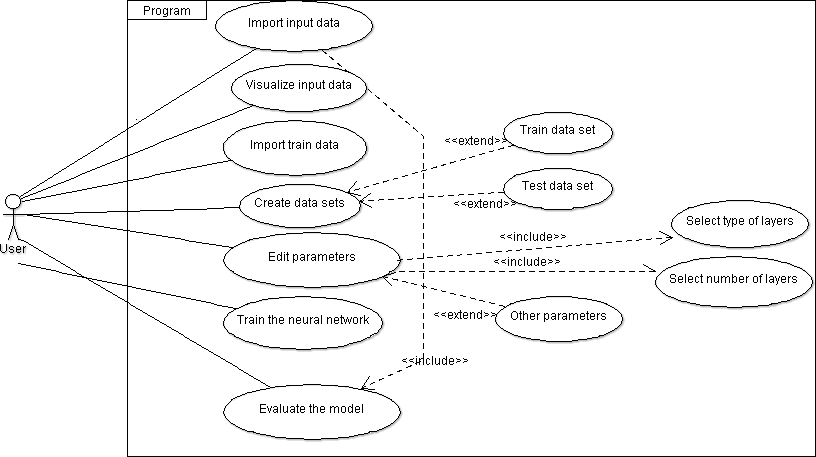
\includegraphics[scale=0.6]{figures/useCase2.png}
    \caption{Use cases diagram}
\end{figure}

\subsection{Non-functional design}

\subsection{Constraints}

\begin{itemize}
\item Platform-compatibility : The app has to be compatible with Linux. If possible, we will try to make it work also with other platforms.
\item Maintainability : We have to develop our application in a way that allows future developers to extend the functionalities. Also, we have to make sure that our app will easily be compatible with future versions of PyTorch.
\end{itemize}

\subsection{Choice of application type}

To develop our application we were thinking about two types of applications. These two choices are a Web-Service, or a regular application.
In order to choose which type of application to develop we drew up a table of advantages and disadvantages.

\begin{itemize}
    \item Web-Service advantages :
    \begin{itemize}
         \item The Web application can be used by all users anywhere and when they want if they are connected to Internet. Furthermore, this facilitates a simple to get a multi-platform application.
        \item The application is always up to date, if it needs an update we only have to update the server whereas a simple application have to be updated on all users' computer. The app is more flexible.
        \item The deployment of the app is easier
        \item It could facilitate the extension of the app to add features
    \end{itemize}
\end{itemize}

 
 \begin{itemize}
    \item Web-Service drawbacks :
    \begin{itemize}
         \item Users need to be connected and to have good network performance (fast and stable) especially in case of big data exchanges. In addition, the server could have to support many users at the same time. Even if the app is running in local, they need to have a good central server, which needs a more complex architecture.
        \item With the same hardware, performances are lower than a native application, we have to exchange data with the server so it must take a long time before getting results especially if we have a lot of data in addition of the time of calculation.
        \item Complex visual effects like drawing a graph could be more complicated to implement
        
    \end{itemize}
\end{itemize}

  \begin{itemize}
    \item Native Application advantages :
    \begin{itemize}
        \item Users don't need an Internet connection.
        \item It has got better performances, better time of calculation, better time of response.(Faster than a Web-Service)
    \end{itemize}
\end{itemize}
\begin{itemize}
    \item Native Application disadvantages :
    \begin{itemize}
        \item Every user have to install the application on his personal computer.
         \item If the application needs an update, we have to upgrade all the computers equipped with the application.
    \end{itemize}
\end{itemize}

\textbf{Our choice :}
Since both options seemed quite equivalent for us, and since having a web-service deployment wasn't a need for the project, we decided to go on to the \textbf{Native Application}. Indeed, this will perfectly allow us to implement all needed features with performance similar to those of PyTorch by itself.

\subsection{Tests}
To make sure the application is working properly, we need to test all features with determined data sets.

Examples of tests :
\begin{itemize}
\item Importing an image and visualise it
\item Importing a set of data, edit its variables and export it
\item Importing a training file, visualize the layers, add a layer, modify a layer, delete a layer, and saving the configuration
\item Testing that the results of classification are always the same as when we use PyTorch in console mode
\item Ergonomics and stability : we have to test that all buttons do an action, that they do the right action, that the application does not crash, and that it is well integrated to the operating system
\end{itemize}
\begin{itemize}
\item In a general way, our tests will consist of being able to use all of PyTorch features with our application, by using default PyTorch test sets.
\end{itemize}

\section{Jupyter NoteBook}
\pagebreak

%---------------------------
%--------- Chapter 5 -------
%---------------------------
\chapter{Project organization}
We have organized our project into five main tasks as follow:

The first one is the Requirements Elicitation, which is all about we have gathered in this document, namely the analysis and main challenges. the analysis of the existing, and the search for the most relevant features to develop in order to fulfill the needs.

The second one, Project Documentation, is about giving feedback of our progress to the client, the teacher, as well as every person who is interested in our project. This will be continued all over the project duration.

There is a Design and an Implementation task too. Since our project is organized in an iterative mode, it means that we will jump from design to programming as many times as it takes to complete all the tasks.

There will be a test phase, in which we will make sure that all of the features we developed work properly. We will try as much as possible to put them in the iterative cycle as well, so we can go from design, to programming, to test, and so on.

\section{Gantt Chart}
\begin{figure}[!ht]
    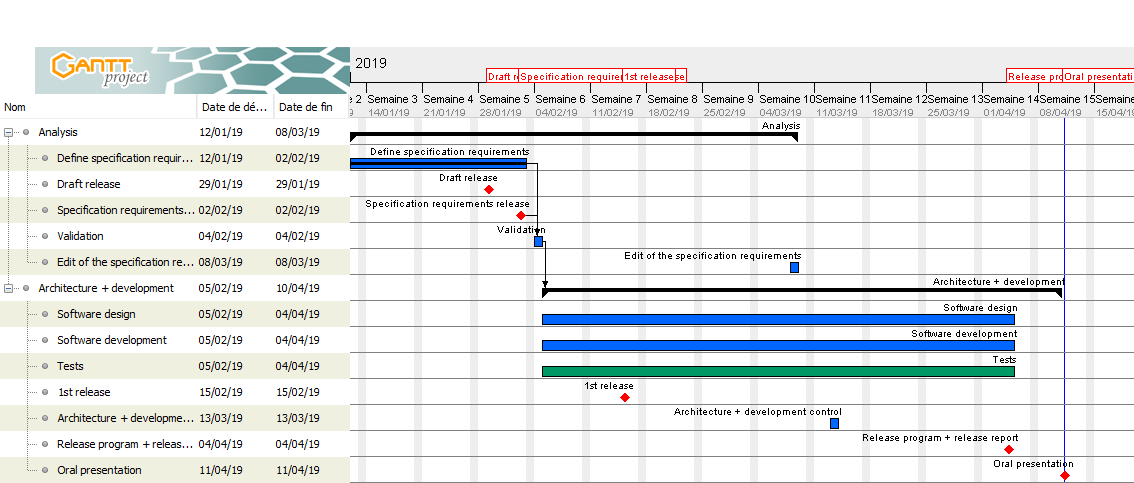
\includegraphics[scale=0.45]{figures/ganttPyTorchfinal.png}
    \caption{Gantt chart}
\end{figure}
\pagebreak


%---------------------------
%----------Bibliograpy------
%---------------------------
\nocite{*}
\bibliographystyle{plain}
\bibliography{references}
\pagebreak

%---------------------------
%---------- Chapter 6-------
%---------------------------
\chapter{Annexes}
\begin{figure}[!ht]
\center
    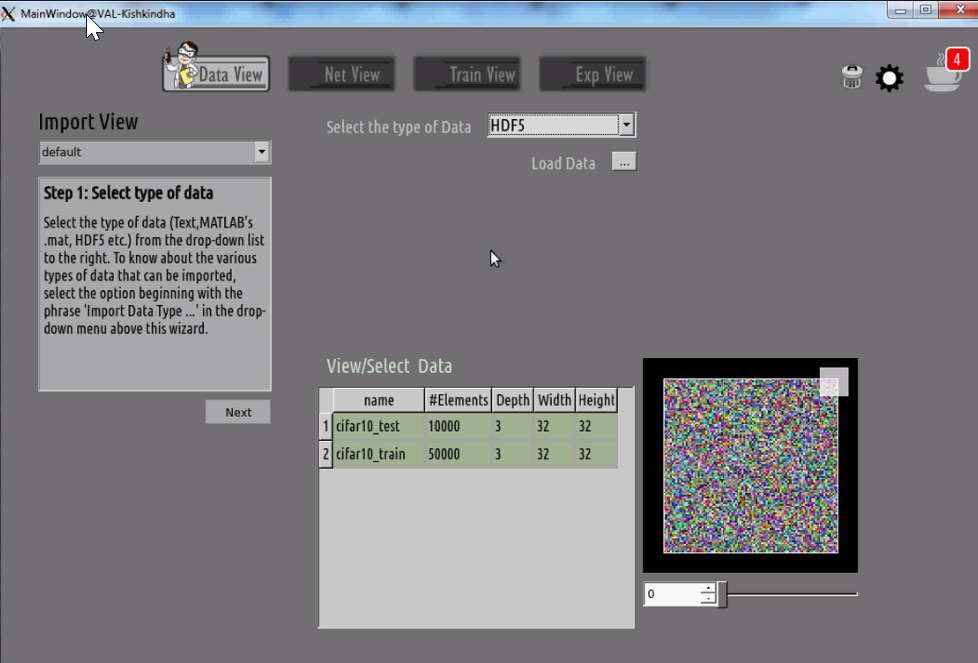
\includegraphics[scale=0.9]{images_expresso/01_data.png}
    \caption{Expresso Data View}
\end{figure}

\begin{figure}[!ht]
\center
    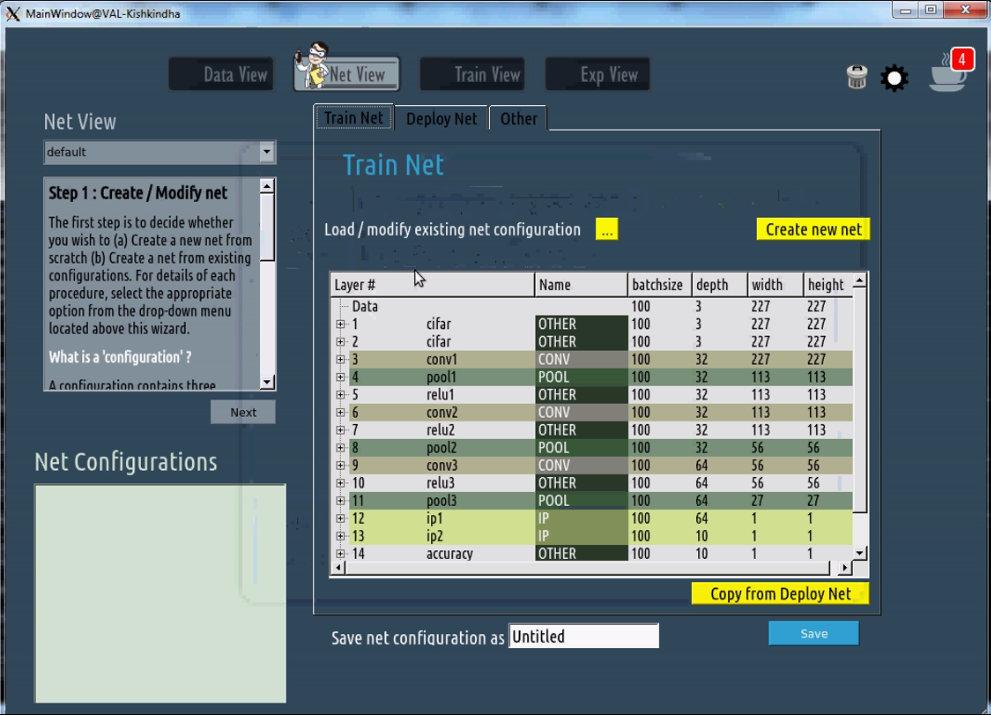
\includegraphics[scale=0.9]{images_expresso/02_net_train_net.png}
    \caption{Expresso Network View (train net part)}
\end{figure}

\begin{figure}[!ht]
\center
    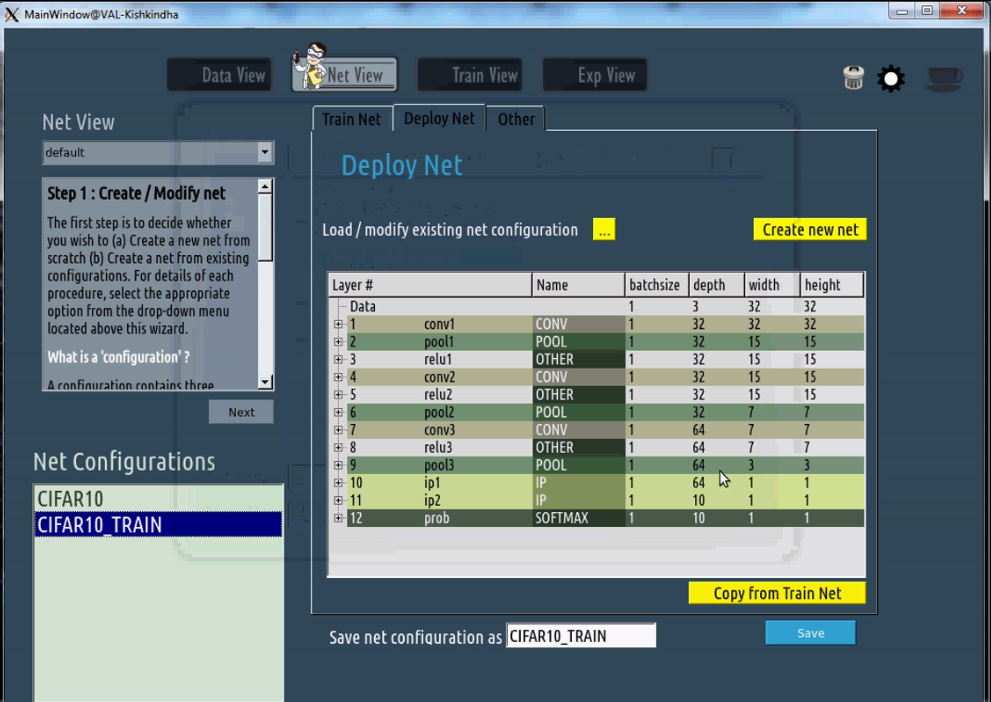
\includegraphics[scale=0.9]{images_expresso/03_net_deploy_net.png}
    \caption{Expresso Network View (deploy net part)}
\end{figure}

\begin{figure}[!ht]
\center
    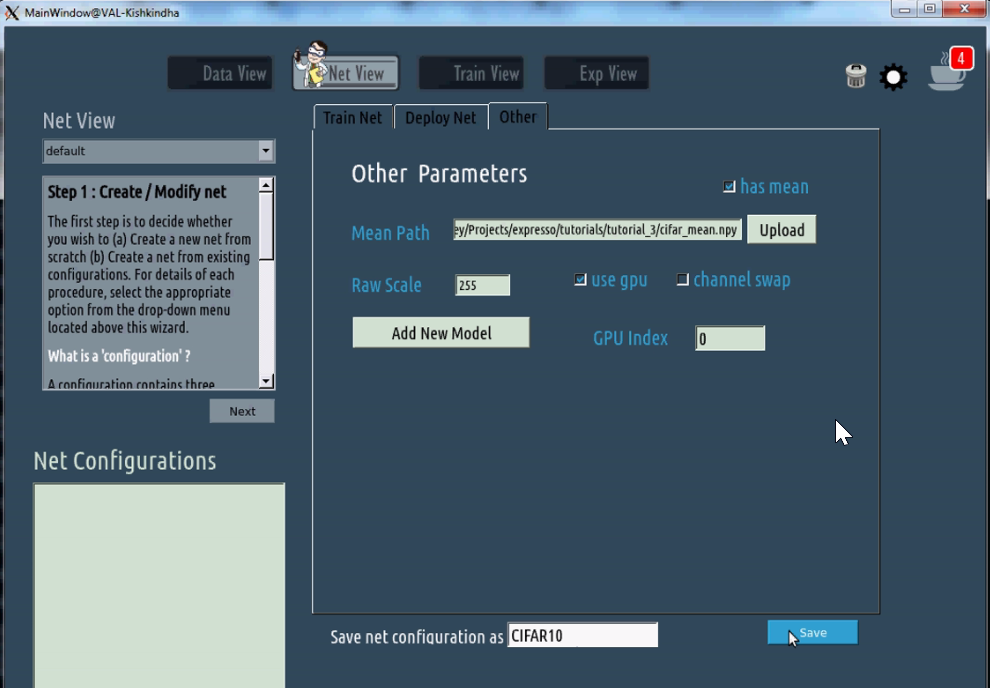
\includegraphics[scale=0.9]{images_expresso/04_net_other.png}
    \caption{Expresso Network View ('other parameters' part)}
\end{figure}

\begin{figure}[!ht]
\center
    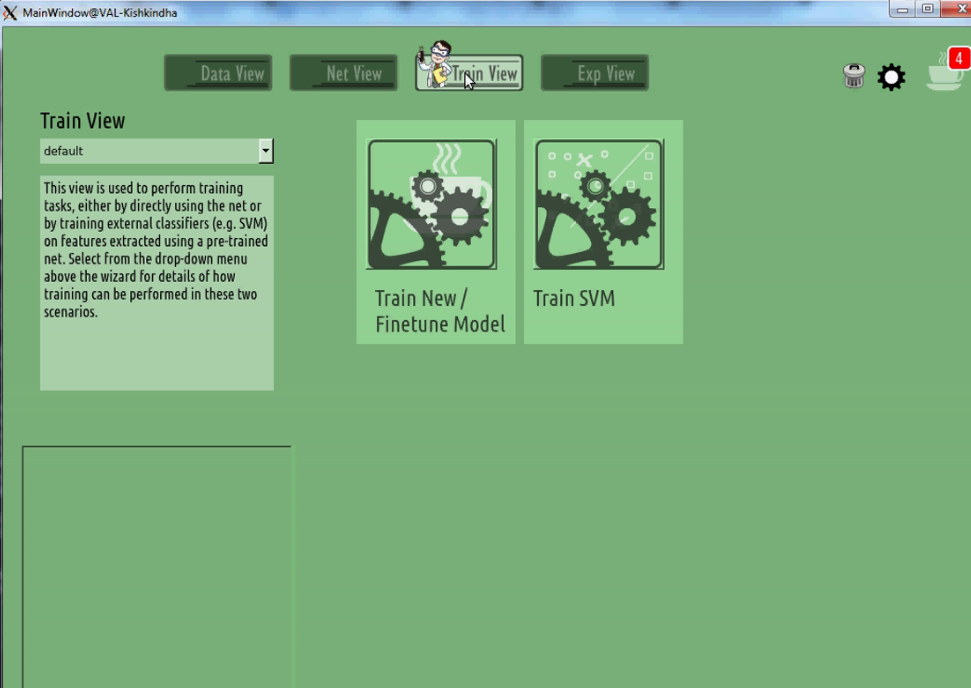
\includegraphics[scale=0.9]{images_expresso/05_train.png}
    \caption{Expresso Train View}
\end{figure}

\begin{figure}[!ht]
\center
    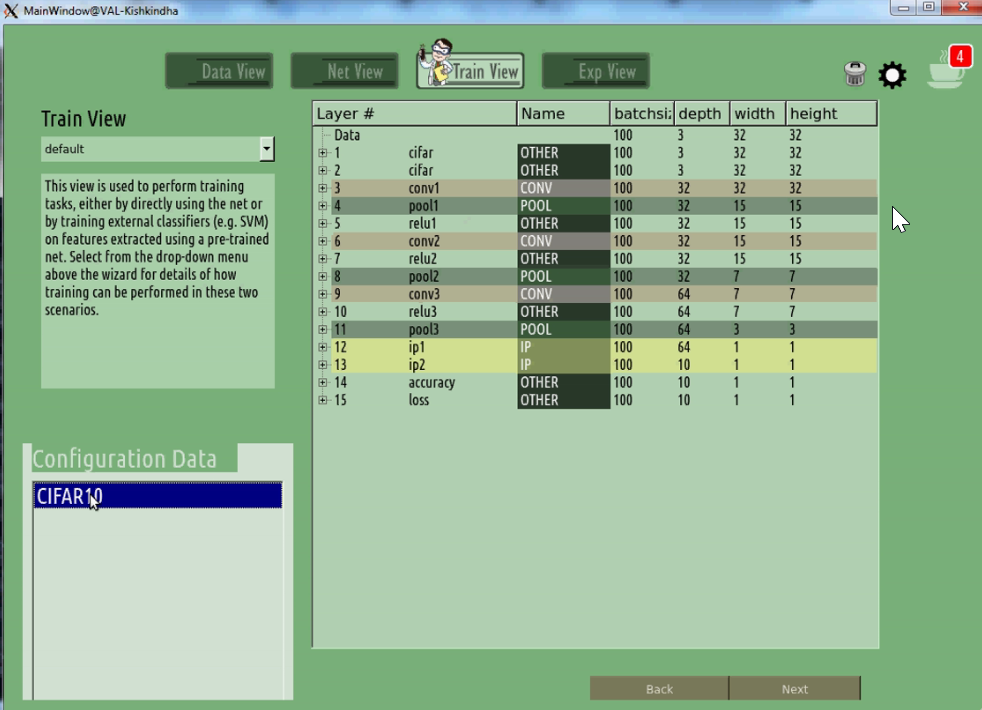
\includegraphics[scale=0.9]{images_expresso/06_train_new.png}
    \caption{Expresso Train View ('Train New/Finetune Model' part)}
\end{figure}

\begin{figure}[!ht]
\center
    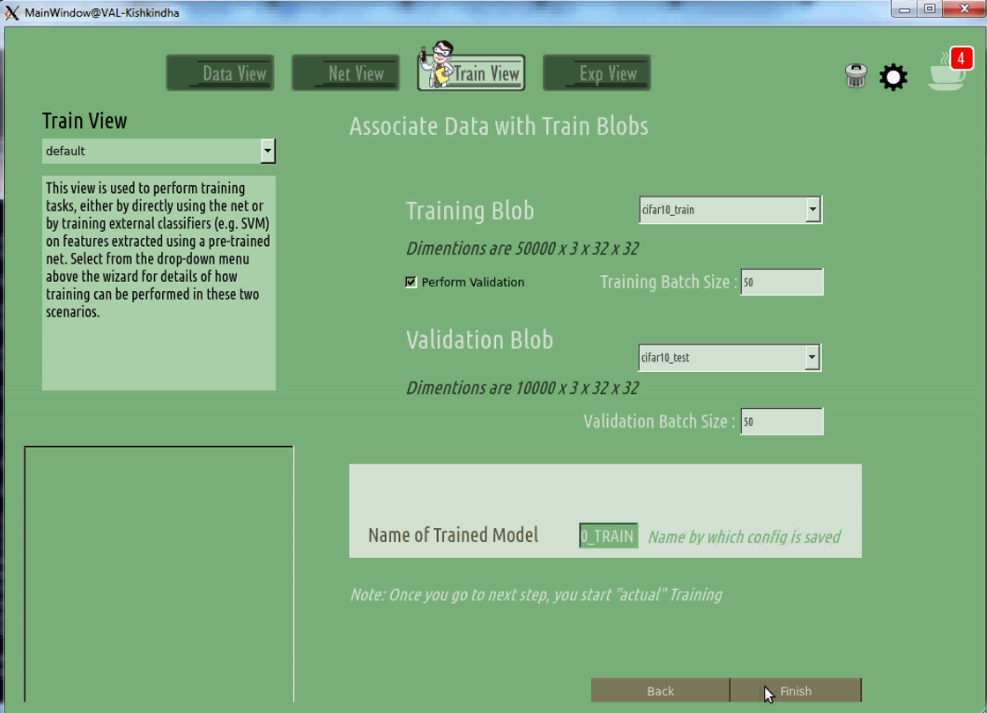
\includegraphics[scale=0.9]{images_expresso/07_train_blobs.png}
    \caption{Expresso Train View ('associate data with train blob' part)}
\end{figure}

\begin{figure}[!ht]
\center
    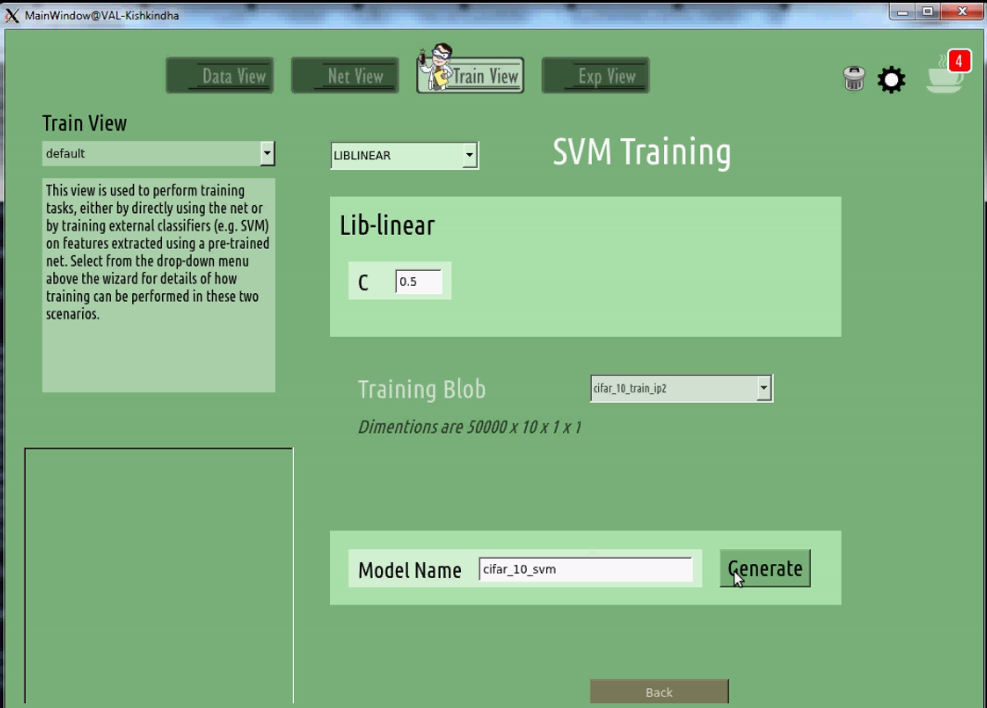
\includegraphics[scale=0.9]{images_expresso/08_train_svm.png}
    \caption{Expresso Train View ('SVM Training' part)}
\end{figure}

\begin{figure}[!ht]
\center
    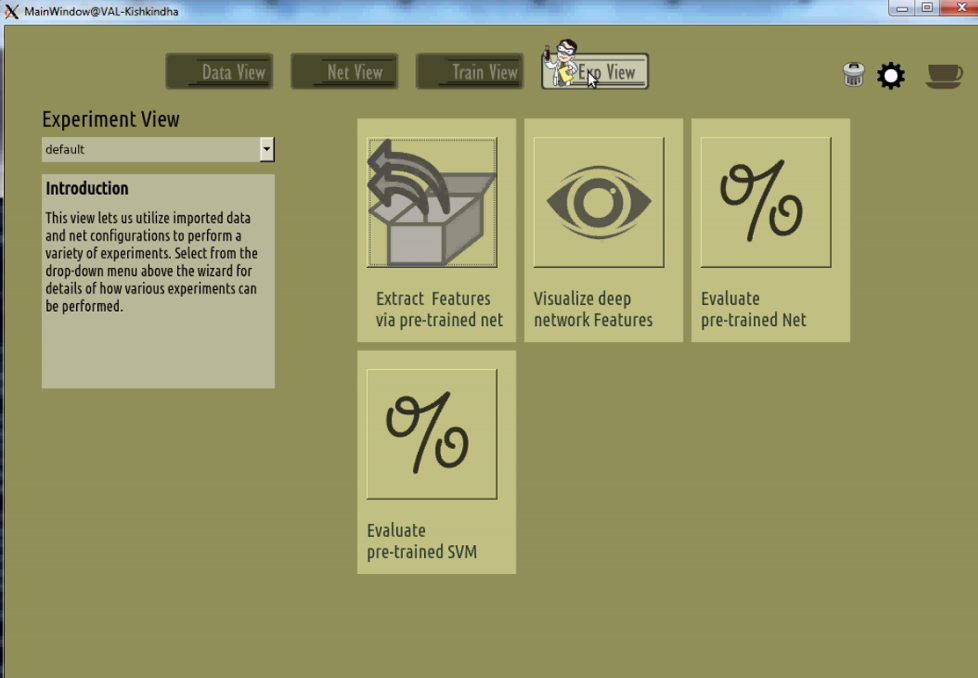
\includegraphics[scale=0.9]{images_expresso/09_exp.png}
    \caption{Expresso Experimental View}
\end{figure}

\begin{figure}[!ht]
\center
    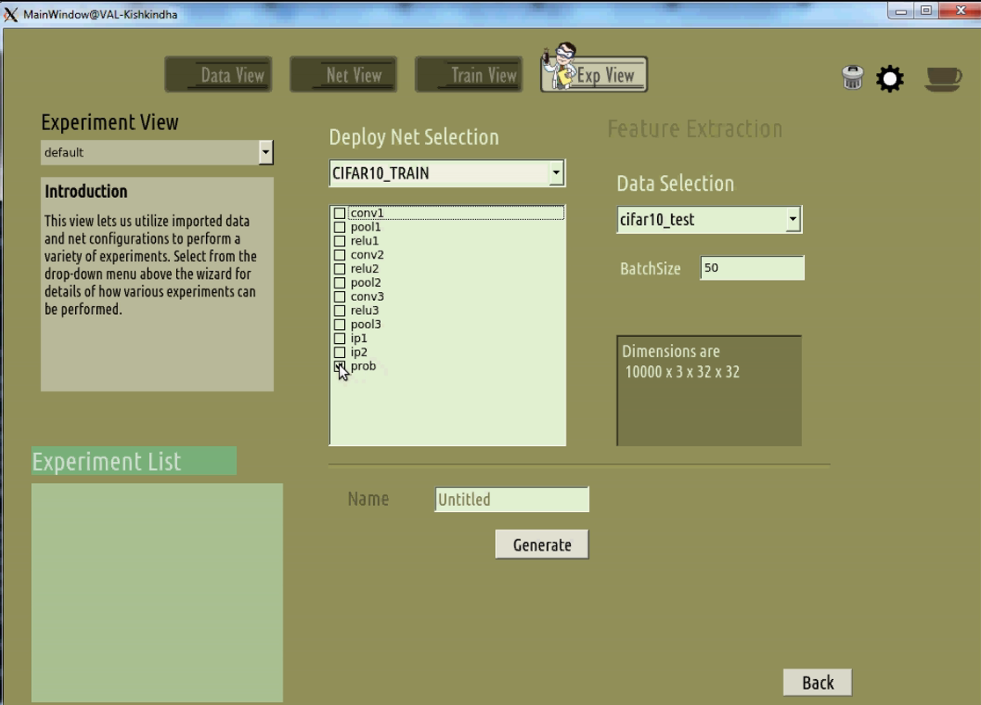
\includegraphics[scale=0.9]{images_expresso/10_exp_feature_extract.png}
    \caption{Expresso Experimental View ('feature extract' part)}
\end{figure}

\begin{figure}[!ht]
\center
    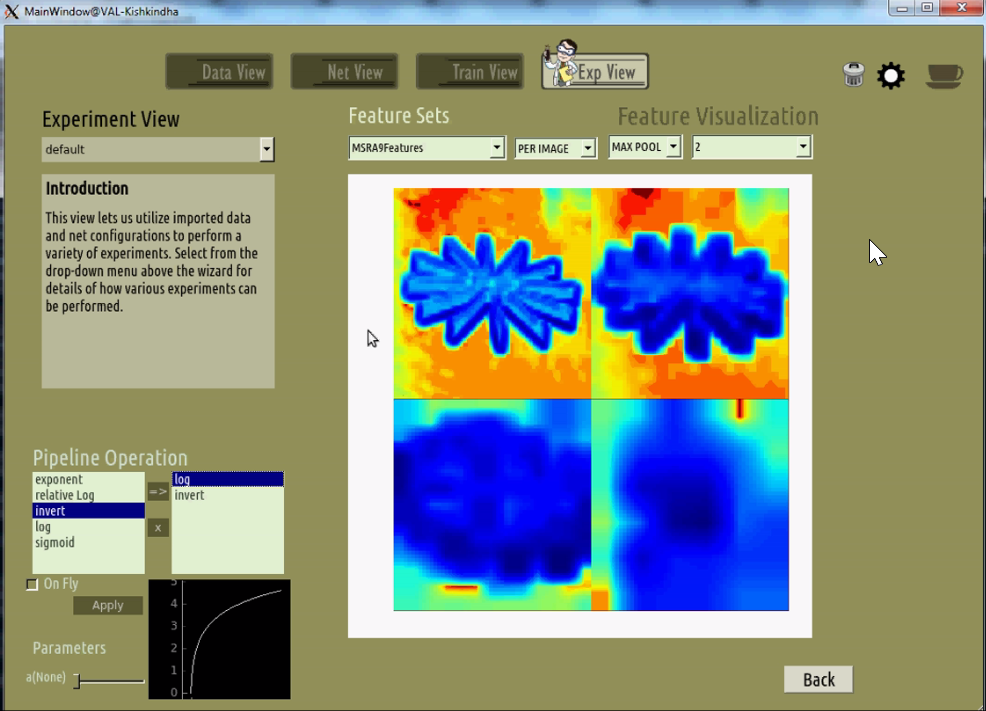
\includegraphics[scale=0.9]{images_expresso/11_exp_visualize.png}
    \caption{Expresso Experimental View ('Visualise features' part)}
\end{figure}

\begin{figure}[!ht]
\center
    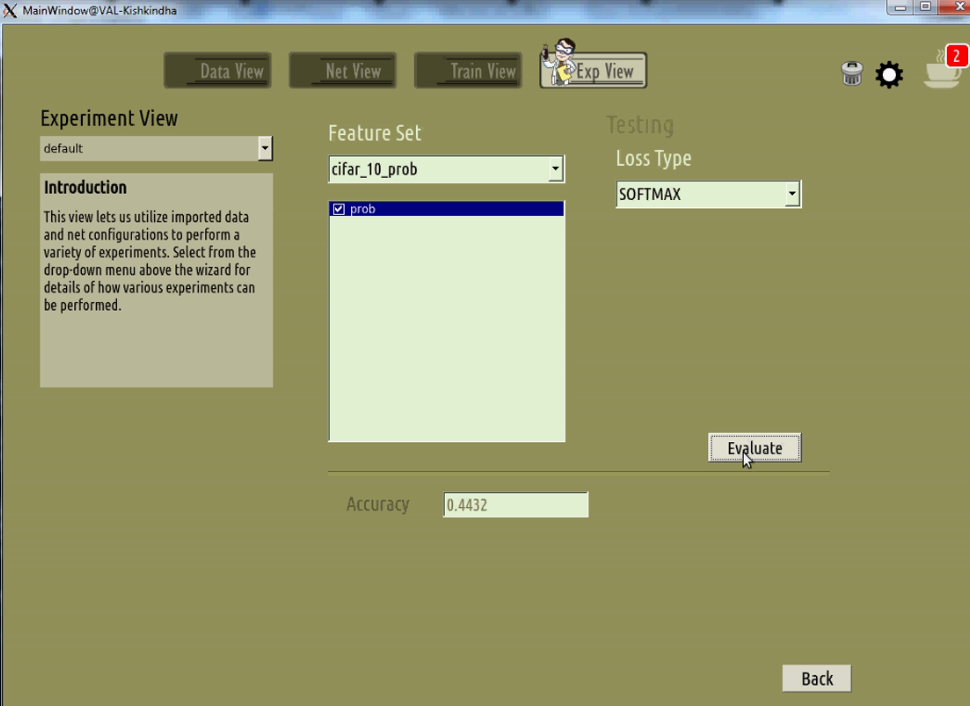
\includegraphics[scale=0.9]{images_expresso/12_exp_evaluate.png}
    \caption{Expresso Experimental View ('Model evaluate' part)}
\end{figure}

\begin{figure}[!ht]
\center
    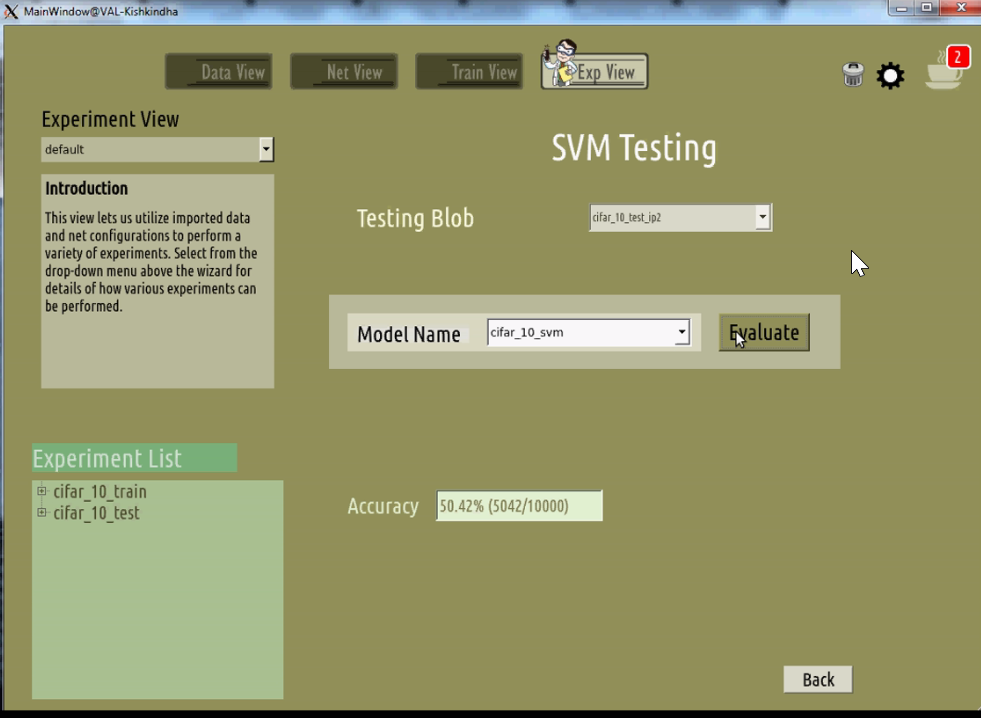
\includegraphics[scale=0.9]{images_expresso/13_exp_svm.png}
    \caption{Expresso Experimental View ('SVM Model evaluate' part)}
\end{figure}

\begin{figure}[!ht]
\center
    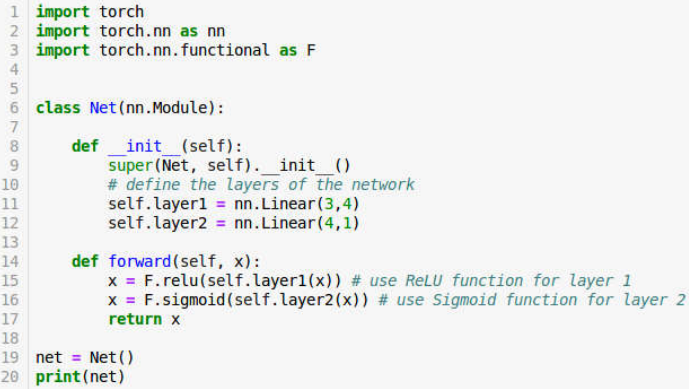
\includegraphics[scale=0.5]{figures/define_nn.png}
    \caption{Define a neural network with PyTorch}
\end{figure}

\end{document}

